
\section{MIP Model}
The MIP formulation was developed with Pyomo, a Python library for writing solver-independent models.
Two models were developed: a base version composed of a 4d array with symmetry breaking and implied constraints, and a better one, optimizing the number of variables featuring circle matching.

\subsection{Variables}
Other than the costants defined in \ref{sec:intro}, the MIP formulation needs two more.
Let $wp = (w,p)$ be the week/period slot $w,p$;
let $m_{i,j} = (i,j)$ be the match played by team $i,j$ with $i<j$:
\[
WP = (\{0, \dots, n-2\},\{0, \dots, \frac{n}{2} - 1\}), \quad M = (\{0, \dots, n-1\},\{0, \dots, n-1\})
\]

\subsubsection*{Decision Variables}
To encode the STS problem we define:
\begin{enumerate}
    \item $\mathbf{Y}_{wp,m} \in \{0,1\}$ \quad $\forall wp \in WP, \; \forall m=(i,j) \in M$ with $i<j$. \\
    $\mathbf{Y}_{wp,m} = 1$ if and only if match $m$ is scheduled in slot $wp$.
    \item $\mathbf{H}_{i,j} \in \{0,1\}$ \quad $\forall (i,j) \in M, \; i<j$. \\
    $\mathbf{H}_{i,j} = 1$ if team $i$ plays at home against $j$, $0$ otherwise.
\end{enumerate}

\subsubsection*{Other Variables}
For the efficiency constraints, we also track whether a team plays in a given period:
\[
\mathbf{Q}_{i,p} \in \{0,1\}, \quad \forall i \in T, \; p \in P,
\]
where $\mathbf{Q}_{i,p} = 1$ if team $i$ has at least one match in period $p$.

\subsection{Objective Function}
\paragraph{Variables}
In order to minimize the maximum imbalance, we need 3 extra variables: 
$\textbf{Home}_{i} \in [0,n-1]$, the number of home matches played by team i
$\textbf{Away}_{i} \in [0,n-1]$, the number of away matches played by team i and
\textbf{Z} $ \in [0,n-1]$, the maximum imbalance across teams

\paragraph{Constraints}
\begin{enumerate}
    \item \textbf{Home games}: 
\[\forall i \in T: \quad \textbf{Home}_{i} = \sum_{j \in T}^{j} \textbf{H}{i,j} + \sum_{j \in T}^{j} (1- \textbf{H}_{j,i}) \quad \text{with $i < j$}\]
    \item \textbf{Away games}: 
\[\forall i \in T: \quad \textbf{Away}_{i} = \sum_{j \in T}^{j} (1- \textbf{H}_{i,j}) + \sum_{j \in T}^{j} \textbf{H}_{j,i} \quad \text{with $i < j$}\]
    \item \textbf{Maximum imbalance}: 
\[
\forall i \in T: \quad |\text{Home}_{i} - \text{Away}_{i}| \leq Z.
\]
\end{enumerate}

\subsection{Constraints}
With circle matching we get a matrix:
\[
\text{presolved}_{w,i,j} = 
\begin{cases}
    \text{1 \quad if the match (i,j) is scheduled for week w}\\
    \text{0 \quad o.w.}
\end{cases}
\]
To take advantage of the precomputed matching schedule, we enforce:
\[\forall w \in W, \forall p \in P, \forall m \in M, m = (i,j): \textbf{Y}_{(w,p),m} \leq \text{presolved}_{w,i,j}\]

Circle matching already takes care of some of the problem constraints, but we have to enforce:
\begin{enumerate}
\item \textbf{One match per w/p slot}: 
\[\forall wp \in WP: \quad\sum_{m \in M}^{m} \textbf{Y}_{wp, m} = 1\]
\item \textbf{One w/p slot per match}: 
\[\forall m \in M: \quad\sum_{wp \in WP}^{wp} \textbf{Y}_{wp, m} = 1\]
\item \textbf{At most 2 matches in the same period}: 
\[
\forall p \in P, \forall k \in T:
\sum_{w \in W}^{w}\sum_{j \in \{k+1\dots n\}}^{j} \textbf{Y}_{(w,p), (k,j)} + 
\sum_{w \in W}^{w}\sum_{i \in \{0\dots k\}}^{i} \textbf{Y}_{(w,p), (i,k)} <= 2
\]
\end{enumerate}

\subsubsection*{Constraints for efficiency}
Especially useful in an optimization environment, this constraint aims to spread the matches of a team in different periods over the scheduling, to get a more balanced result. It also help with symmetry breaking.
\[
    \forall p \in P, \forall i \in T: \quad 2 \cdot \textbf{Q}_{i,p} \geq 
    \sum_{w \in W}^{w}\sum_{j \in \{i+1\dots n\}}^{j} \textbf{Y}_{(w,p), (i,j)} + 
    \sum_{w \in W}^{w}\sum_{j \in \{0\dots i\}}^{j} \textbf{Y}_{(w,p), (j,i)}
\]
\[
    \forall i \in T: \quad \sum_{p \in P}^p \textbf{Q}_{i,p} \geq ceil((n-1)/2)
\]
\subsubsection*{Symmetry breaking constraints}
In this particular model the addition of symmetry breaking constraints did not improve the results, as circle matching already breaks most of the symmetries, and the addition of other constraints only increased the model weight.

\subsection{4D array model}
The simplest possible implementation of the STS problem, developed only for comparison as it is not nearly as efficient as the previous one.
The only decision variable is X, a 4d array $(n-1 \times n/2 \times n \times n)$ of binary values, where each cell represents a match, described as a combination of week, period, team1 and team2. The first team is the one playing home.
The constraints, apart from the necessary ones, include two symmetry-breaking constraints and two implied constraints.
The optimization is performed in the same way as in the previous model.

\subsection{Validation}
The model was implemented in Python using Pyomo 6.9.2. 
The results were obtained by running the models for 3 different solvers:
\textbf{Glpk}, works well for small instances, but does not scale well; \textbf{Cbc}, the most advanced open-source solver; \textbf{Gurobi}: a very efficient commercial solver, used under an academic license.

\subsubsection{Experimental Results}
We tested the MIP formulations on different configurations, using all solvers and both model variants (4D array and Circle Matching, CM). 


\begin{figure}[H]
    \centering
    \begin{subfigure}{\linewidth}
        \centering
        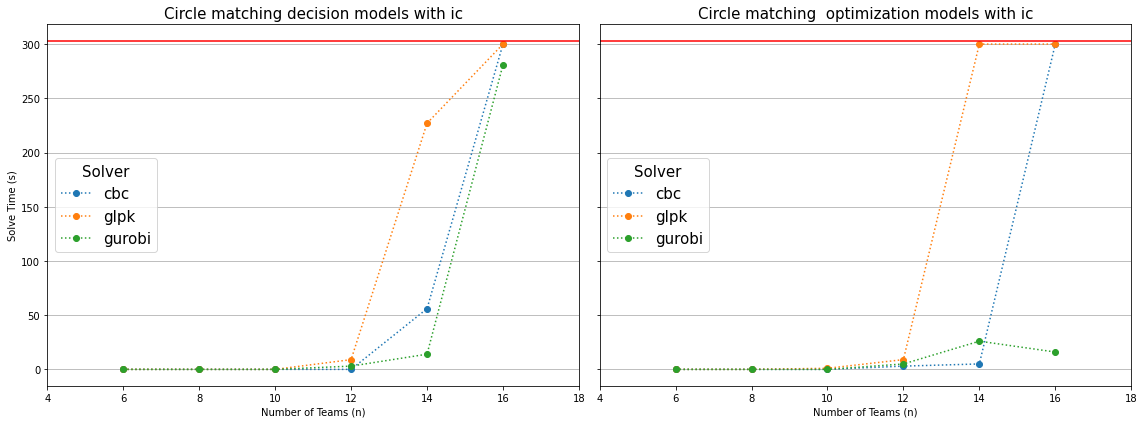
\includegraphics[width=\linewidth]{imgs/plot1.png}
        \caption{Decision vs Optimization}
        \label{fig:mip1}
    \end{subfigure}
\end{figure}

\paragraph{Decision version}
Somewhat counterintuitively, the decision version required on average \emph{more time} to solve (see Figure \ref{fig:mip1}). 
This behavior can be explained by the branch-and-bound exploration of MIP solvers: once the objective is removed, the search tends to focus on constraint satisfaction, which often leads to a larger feasible space and slower convergence.
Moreover, efficiency-oriented constraints, designed to balance the schedule, turned out to be detrimental in this setting.


\begin{table}[H]
    \centering
    \small
    \begin{tabular}{|c|c|c|c|}
    \hline
        \textbf{n} &  \textbf{Model} & \textbf{Solver} & \textbf{Time} \\
    \hline
         8 & 4D & Glpk & 1s \\
         10 & 4D & Glpk & N/A \\
         10 & 4D & Cbc & 4s \\
         12 & 4D & Cbc & N/A \\
         12 & 4D & Gurobi & 23s \\
         12 & CM & Glpk & 17s \\
         12 & CM & Cbc & 14s \\
    \hline
    \end{tabular}
    \begin{tabular}{|c|c|c|c|}
    \hline
        \textbf{n} &  \textbf{Model} & \textbf{Solver} & \textbf{Time} \\
    \hline
        12 & CM & Gurobi & 2s \\
         14 & 4D & Gurobi & 24s \\
         14 & CM & Glpk & N/A \\
         14 & CM & Cbc & 27s \\
         14 & CM & Gurobi & 36s \\
         16 & CM & Cbc & N/A \\
         16 & CM & Gurobi & 72s \\
    \hline
    \end{tabular}
    \caption{Results for the decision problem}
    \text{\small{Efficiency constraints were not enabled here}}
    \label{tab:mip1}
\end{table}

\paragraph{Optimization version}
As expected, the CM model consistently outperformed the 4D array formulation in both solution quality and runtime. This highlights the benefit of a stricter model, with a smaller associated search space.
Table~\ref{tab:mip2} shows how solver performance followed the usual hierarchy: \textbf{Gurobi} was the most efficient, followed closely by \textbf{Cbc}, while \textbf{Glpk} struggled with scalability and often reached the time limit for larger instances. 
Interestingly, though, for some smaller instances Glpk performs better than Cbc.

\begin{table}[H]
    \centering
    \small
    \begin{tabular}{|c|c|c|c|c|}
    \hline
        \textbf{n} &  \textbf{Model} & \textbf{Solver} & \textbf{Time\textbar Obj} \\
    \hline
         10 & 4D & Cbc & 298\textbar1 \\
         10 & 4D & Glpk & 35\textbar1 \\
         10 & 4D & Gurobi & 5\textbar1 \\
         12 & 4D & Cbc/Glpk & N/A \\
         12 & CM & Cbc & 4\textbar1 \\
         12 & CM & Glpk & 10\textbar1 \\
    \hline
    \end{tabular}
    \begin{tabular}{|c|c|c|c|c|}
    \hline
        \textbf{n} &  \textbf{Model} & \textbf{Solver} & \textbf{Time\textbar Obj} \\
    \hline
         12 & CM & Gurobi & 5\textbar1 \\
         14 & CM & Cbc & 5\textbar1 \\
         14 & CM & Glpk & N/A \\
         14 & CM & Gurobi & 26\textbar1 \\
         16 & CM & Cbc & N/A \\
         16 & CM & Gurobi & 16\textbar1 \\
    \hline
    \end{tabular}
    \caption{Results for the optimization problem}
    \text{\small{Efficiency constraints were enabled here}}
    \label{tab:mip2} 
\end{table}